% \chapter{Measurement Results and Discussion}
\chapter{Testování navrženého řešení}
Tato kapitola zahrnuje testování navržené gatewaye senzorové sítě viz. kapitola \ref{Návrh WSN}, napojené přes síť RS485 na infrastrukturu přístupového systému firmy IMA v univerzitní budově univerzity ČVUT za reálného provozu s připojenými koncovými zařízeními senzorové sítě, které souběžně odesílají data. Ze zachyceného provozu dat v síti RS485 je odhadnut maximální počet připojených koncových zařízení souběžně odesílající data v senzorové síti při zachování správné funkce přístupového systému.

Testování je provedeno v jednom bloku patra univerzity, kde je do jednoho kontrolního panelu připojeno dvanáct CKP zařízení přes síť RS485. Každé z nich ovládá jedny dveře, tedy jednu čtečku a dveřní zámek.
Do této sítě RS485 je navíc připojena navržená gateway jako třinácté CKP zařízení.
K této navržené gatewayi senzorové sítě jsou připojena dvě koncová zařízení typu RHF1S001, dostupné na trhu, vyrobené firmou RisingHF, obsahující senzory teploty a vlhkosti. Pro tento test jsou nakonfigurovány k odesílání dat ze senzorů s intervalem 5 minut.

Gateway a CKP zařízení jsou zapojena dle blokového schematu v obrázku \ref{fig:ACS architecture IMA with geteway}.
Konkrétní rozmístění stávajících dvanácti CKP zařízení, gatewaye a dvou koncových zařízení senzorové sítě v testovaných prostorách budovy je zobrazeno v obrázku \ref{fig:CorridorFloorPlan}.

\begin{figure*}[!ht]
    \centering
    \includegraphics[width=1\textwidth]{5patro}
    \caption{Rozmístění koncových zařízení sítě a zařízení CKP v testovaných prostorách budovy}
    \label{fig:CorridorFloorPlan}
\end{figure*}

Testování probíhalo od 21. září do 31. října, tedy v době přítomnosti studentů a zaměstnanců v testovaných prostorách. 
Po tuto dobu testování byly zaznamenávány přenášené pakety síti RS485, kontrolní panel přijal 1~876~978 paketů (14~074~522 B) a odeslal 1~101~556 paketů (8~295~219 B), dohromady tedy 2~978~534 paketů (22~369~741 B).
Z naměřených hodnot byla provedena metoda frekvenční analýzy. Z přenesených paketů byly nejdelší 3 o velikostí 40 bytů.
S ohledem na celkové množství paketů je to zanedbatelné množství, tj. 1,3E-04 \%.
Avšak vzhledem k povaze systému, tedy systému s primární funkcí řízení přístupu do omezených oblastí, se za nejhorší scénář považuje nepřekonatelný limit velikosti paketu.

Maximální počet koncových zařízení připojených ke gatewayi při kterém není ovlivněn stávájící přístupový systém je možné vypočítat z rychlosti přenosu dat v síti RS485. 
Tato rezerva rychlosti přenosu dat je uvažována za účelem ochrany přístupového systému před dysfunkcí nebo poruchou, například před dlouhým čekáním na otevření dveří.

\begin{longtable} {|c|r|}
% \footnotesize
\caption{Frekvenční analýza délky paketu} 
\label{tab:FreqAnalysis} \\
            \hline
    Délka paketu &  Počet \\ \hline
    \textbf{7}  &  \textbf{2~216~098}  \\
    8  &   619~127   \\
    9  &         3   \\
    11 &    58~393   \\
    13 &    58~620   \\
    16 &         1   \\
    18 &         2   \\
    \textbf{19} &    \textbf{26~286}   \\
    23 &         1   \\
    40 &         3   \\
    \hline
\end{longtable}

\newpage
\begin{figure*}[h]
    \centering
    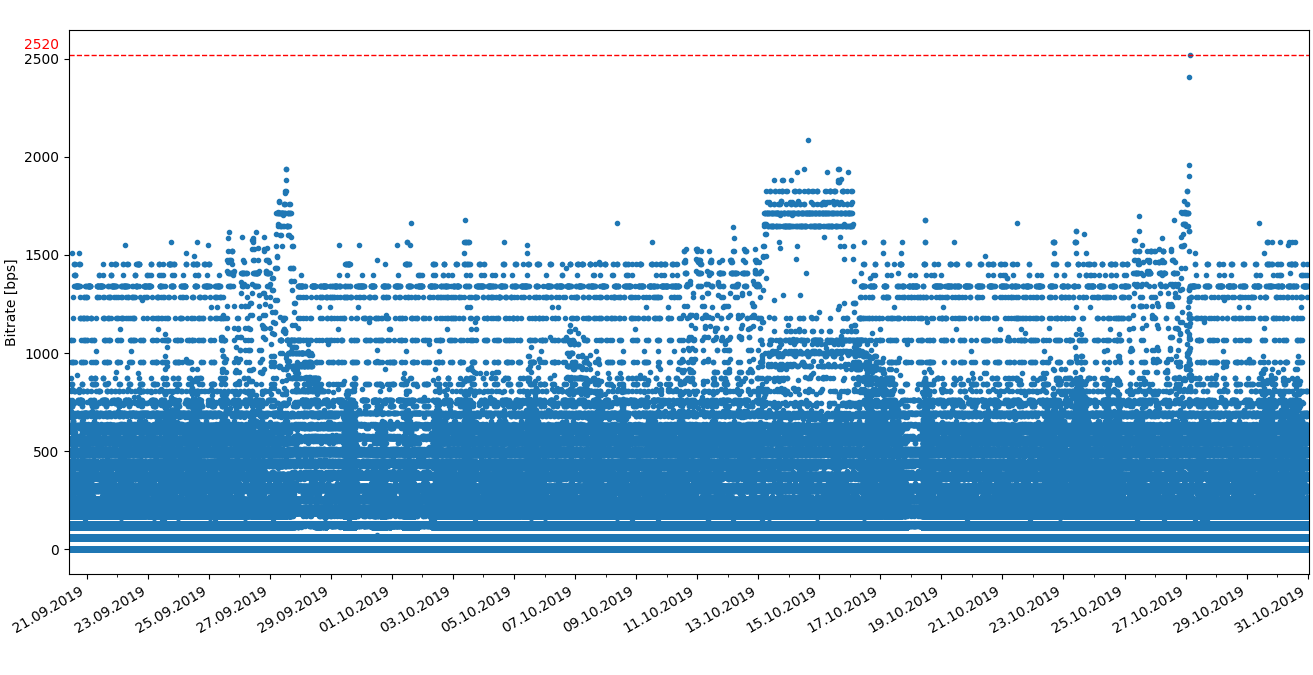
\includegraphics[width=1\textwidth]{03-dr-measured}
    \caption{Měřená rychlost přenosu dat [bps] v síti RS485 během doby testování}
    % \caption{Measured data rate in [bps] in RS485 network during long-term operation test}
    \label{fig:PacketLengthMeasuredAll}
\end{figure*}

Na základě frekvenční analýzy uvedené v tabulce \ref{tab:FreqAnalysis} a IMA know-how, pakety přenášející data z koncových zařízení jsou dlouhé 19 bytů a pakety potvrzení IMA protokolu jsou dlouhé 7 bytů. Alespoň dva pakety jsou potřeba k přenesení dat z koncových zařízení přes síť RS485, tj. paket s daty koncového zařízení a paket potvrzení.

V obrázku \ref{fig:PacketLengthMeasuredAll} jsou dvě důležité charakteristiky, maximální délka paketu 
(červená přerušovaná čára) a medián délky paketu (červená nepřerušovaná čára), určeny frekvenční analýzou v tabulce \ref{tab:FreqAnalysis}. 
Průměrné zatížení provozu kanálu sítě RS485 je 6,38 pps, tj. 0,85 Bps.
%shows lengths of captured packet  during
%Median of packet length is determined by using frequency analysis method, as shown in Tab. \ref{tab:FreqAnalysis}.
% 7,51 Byte --> simple arithmetic mean


Z testování provozu jsou zachyceny délky přenášených paketů ($ l $) s časovou přesností na tisícinu sekundy. Údaje o čase jsou převedeny na jednotky sekund pomocí funkce sum, aby byly získány data jako bitová rychlost v bitech za sekundu (bps),
V obrázku \ref{fig:PacketLengthMeasuredAll} červená přerušovaná čára s hodnotou 2520~bps) ukazuje jeden sekundový interval ve kterém součet přenesených paketů v síti RS485.
Na základě podrobných znalosti protokolu IMA se ukazuje, že je využito méně než 20\% kapacity sítě RS485 
%This limit state is caused by data communication of two sensor nodes that occupied 2\% of capacity of used RS485 network.

Aby bylo zabráněno přetížení sítě RS485, maximální počet koncových zařízení připojených ke gatewayi $ S_{MAX} $ je možné vypočítat vztahem:

\begin{equation}
S_{MAX} = \frac{\frac{\frac{v_{485}}{B}}{l_{MAX}} - R}{P}
\label{equ:max-count-of-sensors}
\end{equation}

kde:

\begin{tabular}{l @{  } l}
$v_{485}$ & rychlost přenosu dat v síti RS485 [bps]\\
 B        & počet bitů v bytu (pro přepočítání rychlosti přenosu dat na byty) \\
$l_{MAX}$ & maximální délka paketu \\
 R        & rezerva rychlosti přenosu dat [\%]\\
 P        & počet paketů k přenesení dat z koncového zařízení \\
\end{tabular}


S ohledem na výše uvedené limity, navržené rezervy a rychlosti přenosu dat v síti RS485 je vypočítán maximální počet koncových zařízení senzorové sítě, které souběžně odesílají data přes síť RS485 viz. tabulka \ref{tab:max-sensor-nodes}.

Použité hodnoty pro výpočet jsou:

\begin{tabular}{l @{ $=$ } l}
$v_{485}$ & RS485 network data rate \\
 B        & 8 \\
$l_{MAX}$ & 40 \\
 P        & 2 \\
\end{tabular}



\begin{longtable} {|l|llll|}
% \footnotesize
\caption{Maximální počet připojených koncových zařízení v senzorové síti souběžně odesílající data skrze síť RS485 s určitou    
    rezervou}      \label{tab:max-sensor-nodes} \\
    \hline

    \textbf{RS485 rychlost přenosu dat} &       \multicolumn{4}{c|}{\textbf{Rezerva R}}	  	    \\

    $v_{485}$ {[bps]}  &	0 \%	&	10 \%	&	20 \%	&	30 \%  \\ \hline

    1200~~~ &    1	&    1	&    1	&    1 \\
    2400~~~ &    3	&    3	&    3	&    2 \\
    4800~~~ &    7	&    6	&    6	&    5 \\
    9600~~~ &   15	&   13	&   12	&   10 \\
    19200~~~ &   30	&   27	&   24	&   21 \\
    38400~~~ &   60	&   54	&   48	&   42 \\
    57600~~~ &   90	&   81	&   72	&   63 \\
    115200~~~ &  180	&  162	&  144	&  126 \\
    230400~~~ &  360	&  324	&  288	&  252 \\
    460800~~~ &  720	&  648	&  576	&  504 \\
    921600~~~ & 1440	& 1296	& 1152	& 1008 \\
    \hline

\end{longtable}


Např. v senzorové síti může být až 54 koncových zařízení připojených ke gatewayi, která je napojena na síť RS485 s přenosovou rychlostí 38400~bps a rezervou 10 \% nebo 42 koncových zařízení s přenosovou rychlostí 38400~bps a rezervou 30 \%.
Tento výsledek ukazuje, že jeden blok patra univerzity, tj. jedna síť RS485 je schopna fungovat s desítkami koncovými zařízeními senzorové sítě souběžně vysílající data s dostatečnou rezervou chránící přístupový systém. 






%%%%%%%%%%%%%%%%%%%%%%%%%%%%%%%%%%%%%%%%%%%%%%%%%%%%%%%%%%%%%%%%%%%%%%%%%%%%%%%%%%%%%%%
%       NOT USED
%%%%%%%%%%%%%%%%%%%%%%%%%%%%%%%%%%%%%%%%%%%%%%%%%%%%%%%%%%%%%%%%%%%%%%%%%%%%%%%%%%%%%%%
% The heavy traffic test simulates data transmission in the RS485 network as evidence of theoretically calculated values as shown in Tab \ref{tab:max-sensor-nodes}.

% \begin{figure}[!ht]
    % \centering
    % 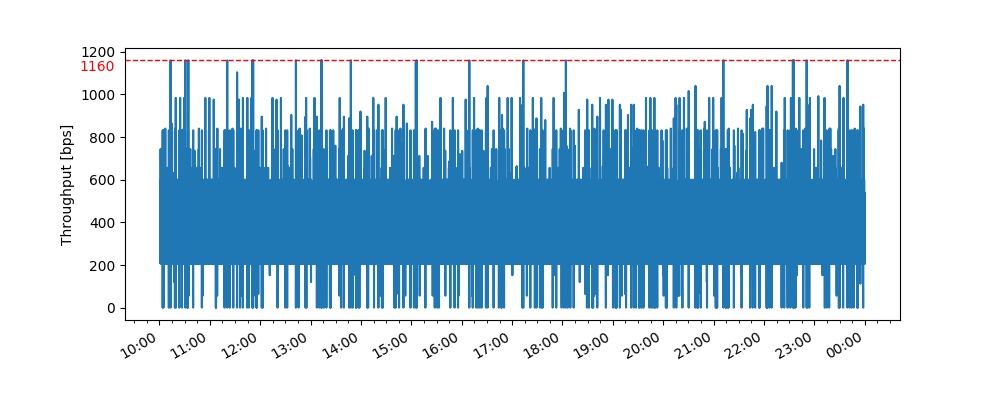
\includegraphics[width=.5\textwidth]{03-tp-simul}
    % \caption{RS485 datarates in simulation of heavy data traffic}
    % \label{fig:heavySimulation}
% \end{figure}

% This test simulated the transmission of more than 190~000 commands from 300 sensor nodes every 5 minutes simultaneously for 12 hours time period. The highest datarate achieved during simulation is 1160~bps, Fig \ref{fig:heavySimulation} red dashed line.

%!!! Tady to mozna chce frekvencni analyzu GW, at vis, jak jsou dlouhe pakety, pak nemusis hadat, nebo napis, ze max. delka je 19 bytů.

%Considering the worst case, ie packets with length of 40 Bytes, we have analytically calculated the maximum number of sensors a network can transmit based on the network transmission rate.

%\textbf{!!! Limit RS485: up to 32 transceivers on the serial bus !!! My vsak mame senzory pres LoRa ...Jo, ale to je fyzicky, to splnujeme, mame jich 13 :-)}
%datasheet: https://www.sparkfun.com/datasheets/Components/General/sp3485CN-LTR.pdf

%Space for peaks 10\% --> maximum packet rate is 324 pps
%Data measured in testing procedure shows Fig.

%\begin{table}[h]
%\centering
%\footnotesize
%\caption{Simple analytics of measured data}
%\begin{tabular}{lr}
%\textbf{Packet length} & \textbf{Bytes} \\ \hline
%Minimum   &   7 B     \\
%Maximum   &  40 B     \\
%mean      &   7,51 B  \\
%Median    &   7 B     \\
%\end{tabular}
%\label{tab: simple-analytics}
%\end{table}


%---
% tabulka, rezervy 10%, 30% ...
% Zjistit kolik sensoru muze byt na sbernici 485.
% popis os co  je co
